\documentclass[tikz,border=4pt]{standalone}
\usepackage{tikz}
\usepackage{xcolor}
\usepackage{amsmath}

\definecolor{mleblue}{HTML}{2A78D6}
\definecolor{mleorange}{HTML}{EB6834}
\definecolor{mlegray}{HTML}{C3C2B7}
\definecolor{mleink}{HTML}{0B0B0B}
\definecolor{mlesub}{HTML}{52514E}
\definecolor{mlemut}{HTML}{898781}
\definecolor{mlegrid}{HTML}{E1E0D9}
\definecolor{mlesurf}{HTML}{FCFCFB}

\begin{document}
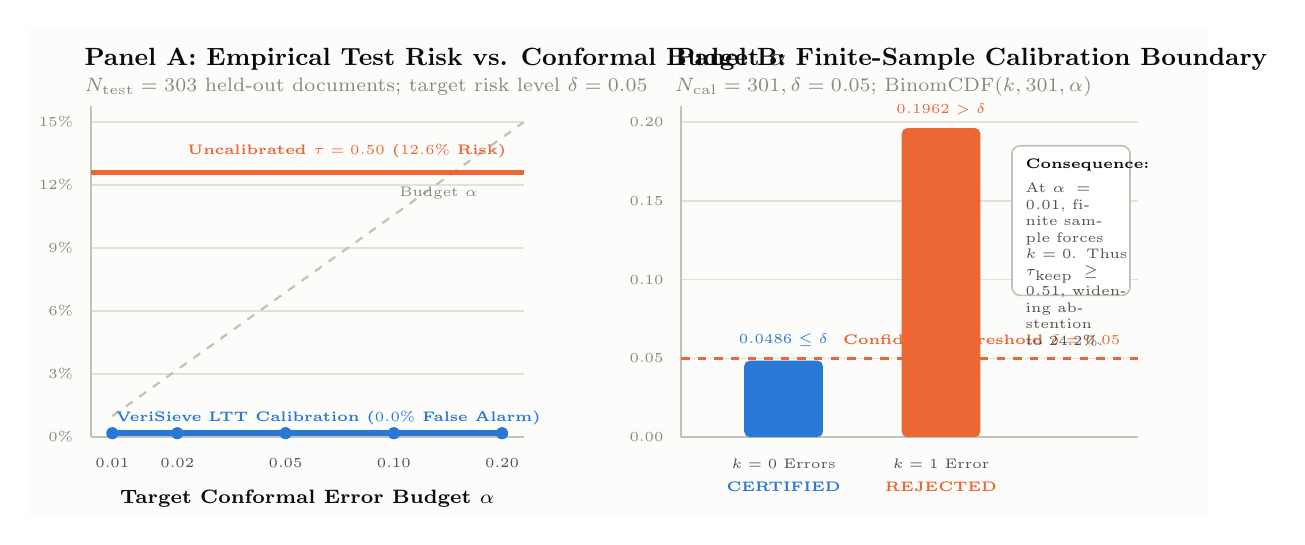
\begin{tikzpicture}[x=1cm, y=1cm, font=\sffamily]
  % Background surface
  \fill[mlesurf] (-0.8, -1.0) rectangle (14.2, 5.2);

  % ================= PANEL A =================
  \begin{scope}[shift={(0,0)}]
    \node[anchor=west, text=mleink, font=\bfseries\small] at (-0.2, 4.8) {Panel A: Empirical Test Risk vs. Conformal Budget $\alpha$};
    \node[anchor=west, text=mlemut, font=\scriptsize] at (-0.2, 4.45) {$N_{\text{test}} = 303$ held-out documents; target risk level $\delta = 0.05$};

    % Grid lines
    \draw[mlegrid, line width=0.5pt] (0,0) -- (5.5,0);
    \draw[mlegrid, line width=0.5pt] (0,0.8) -- (5.5,0.8);
    \draw[mlegrid, line width=0.5pt] (0,1.6) -- (5.5,1.6);
    \draw[mlegrid, line width=0.5pt] (0,2.4) -- (5.5,2.4);
    \draw[mlegrid, line width=0.5pt] (0,3.2) -- (5.5,3.2);
    \draw[mlegrid, line width=0.5pt] (0,4.0) -- (5.5,4.0);

    % Y Axis labels
    \node[anchor=east, text=mlemut, font=\tiny] at (-0.1, 0) {0\%};
    \node[anchor=east, text=mlemut, font=\tiny] at (-0.1, 0.8) {3\%};
    \node[anchor=east, text=mlemut, font=\tiny] at (-0.1, 1.6) {6\%};
    \node[anchor=east, text=mlemut, font=\tiny] at (-0.1, 2.4) {9\%};
    \node[anchor=east, text=mlemut, font=\tiny] at (-0.1, 3.2) {12\%};
    \node[anchor=east, text=mlemut, font=\tiny] at (-0.1, 4.0) {15\%};

    % Axes
    \draw[mlegray, line width=0.8pt] (0,0) -- (5.5,0);
    \draw[mlegray, line width=0.8pt] (0,0) -- (0,4.2);

    % Theoretical diagonal budget line alpha = risk
    \draw[mlegray, dashed, line width=0.8pt] (0.275, 0.267) -- (5.5, 4.0);
    \node[anchor=south west, text=mlemut, font=\tiny] at (3.8, 2.9) {Budget $\alpha$};

    % Uncalibrated baseline tau = 0.50 (12.6% violation)
    \draw[mleorange, line width=1.5pt] (0, 3.36) -- (5.5, 3.36);
    \node[anchor=south east, text=mleorange, font=\tiny\bfseries] at (5.4, 3.42) {Uncalibrated $\tau = 0.50$ ($12.6\%$ Risk)};

    % VeriSieve LTT Empirical Risk line (0.0% across all alpha)
    \draw[mleblue, line width=2pt] (0.275, 0.05) -- (5.225, 0.05);
    \foreach \x/\val in {0.275/0.01, 1.1/0.02, 2.475/0.05, 3.85/0.10, 5.225/0.20} {
      \fill[mleblue] (\x, 0.05) circle (2.2pt);
    }
    \node[anchor=north west, text=mleblue, font=\tiny\bfseries] at (0.2, 0.45) {VeriSieve LTT Calibration ($0.0\%$ False Alarm)};

    % X Axis labels
    \node[anchor=north, text=mlesub, font=\tiny] at (0.275, -0.15) {0.01};
    \node[anchor=north, text=mlesub, font=\tiny] at (1.1, -0.15) {0.02};
    \node[anchor=north, text=mlesub, font=\tiny] at (2.475, -0.15) {0.05};
    \node[anchor=north, text=mlesub, font=\tiny] at (3.85, -0.15) {0.10};
    \node[anchor=north, text=mlesub, font=\tiny] at (5.225, -0.15) {0.20};
    \node[anchor=north, text=mleink, font=\scriptsize\bfseries] at (2.75, -0.55) {Target Conformal Error Budget $\alpha$};
  \end{scope}

  % ================= PANEL B =================
  \begin{scope}[shift={(7.5,0)}]
    \node[anchor=west, text=mleink, font=\bfseries\small] at (-0.2, 4.8) {Panel B: Finite-Sample Calibration Boundary};
    \node[anchor=west, text=mlemut, font=\scriptsize] at (-0.2, 4.45) {$N_{\text{cal}} = 301, \delta = 0.05$; $\operatorname{BinomCDF}(k, 301, \alpha)$};

    % Grid lines
    \draw[mlegrid, line width=0.5pt] (0,0) -- (5.8,0);
    \draw[mlegrid, line width=0.5pt] (0,1.0) -- (5.8,1.0);
    \draw[mlegrid, line width=0.5pt] (0,2.0) -- (5.8,2.0);
    \draw[mlegrid, line width=0.5pt] (0,3.0) -- (5.8,3.0);
    \draw[mlegrid, line width=0.5pt] (0,4.0) -- (5.8,4.0);

    % Y Axis labels
    \node[anchor=east, text=mlemut, font=\tiny] at (-0.1, 0) {0.00};
    \node[anchor=east, text=mlemut, font=\tiny] at (-0.1, 1.0) {0.05};
    \node[anchor=east, text=mlemut, font=\tiny] at (-0.1, 2.0) {0.10};
    \node[anchor=east, text=mlemut, font=\tiny] at (-0.1, 3.0) {0.15};
    \node[anchor=east, text=mlemut, font=\tiny] at (-0.1, 4.0) {0.20};

    % Axes
    \draw[mlegray, line width=0.8pt] (0,0) -- (5.8,0);
    \draw[mlegray, line width=0.8pt] (0,0) -- (0,4.2);

    % Critical threshold delta = 0.05
    \draw[mleorange, dashed, line width=1.2pt] (0, 1.0) -- (5.8, 1.0);
    \node[anchor=south east, text=mleorange, font=\tiny\bfseries] at (5.7, 1.05) {Confidence Threshold $\delta = 0.05$};

    % Bars for Binomial CDF at alpha = 0.01:
    % k = 0: BinomCDF = 0.0486 <= 0.05 (Valid!)
    % k = 1: BinomCDF = 0.1962 > 0.05 (Violates delta!)
    % k = 2: BinomCDF = 0.4200 > 0.05
    \fill[mleblue, rounded corners=2pt] (0.8, 0) rectangle (1.8, 0.972);
    \node[anchor=south, text=mleblue, font=\tiny\bfseries] at (1.3, 1.02) {$0.0486 \le \delta$};
    \node[anchor=north, text=mlesub, font=\tiny] at (1.3, -0.15) {$k=0$ Errors};
    \node[anchor=north, text=mleblue, font=\tiny\bfseries] at (1.3, -0.45) {CERTIFIED};

    \fill[mleorange, rounded corners=2pt] (2.8, 0) rectangle (3.8, 3.924);
    \node[anchor=south, text=mleorange, font=\tiny\bfseries] at (3.3, 3.97) {$0.1962 > \delta$};
    \node[anchor=north, text=mlesub, font=\tiny] at (3.3, -0.15) {$k=1$ Error};
    \node[anchor=north, text=mleorange, font=\tiny\bfseries] at (3.3, -0.45) {REJECTED};

    % Consequence annotation box
    \draw[mlegray, fill=white, rounded corners=3pt, line width=0.6pt] (4.2, 1.8) rectangle (5.7, 3.7);
    \node[anchor=north west, text=mleink, font=\tiny\bfseries] at (4.25, 3.65) {Consequence:};
    \node[anchor=north west, text=mlesub, font=\fontsize{5}{6}\selectfont, text width=1.3cm] at (4.25, 3.35) {At $\alpha=0.01$, finite sample forces $k=0$. Thus $\tau_{\text{keep}} \ge 0.51$, widening abstention to 24.2\%.};
  \end{scope}
\end{tikzpicture}
\end{document}
